\documentclass{acmtog}

\acmVolume{VV}
\acmNumber{N}
\acmYear{2012}
\acmMonth{February}
\acmArticleNum{XXX}  
\acmdoi{10.1145/XXXXXXX.YYYYYYY}

%\acmVolume{28}
%\acmNumber{4}
%\acmYear{2009}
%\acmMonth{August}
%\acmArticleNum{106}  
%\acmdoi{10.1145/1559755.1559763}

\usepackage[pdfborder={0 0 0}]{hyperref}
\usepackage[retainorgcmds]{IEEEtrantools}
\usepackage{relsize}

\begin{document}

\markboth{A.C. Macedo | M. Palhas | P. Costa}{Integrated Project}

\title{Integrated Project: Vision controlled camera} % title

\author{
Ana Catarina Macedo --- {\ttfamily a54773@alunos.uminho.pt}\\
Miguel Palhas --- {\ttfamily pg19808@alunos.uminho.pt}\\
Pedro Costa --- {\ttfamily pg19830@alunos.uminho.pt}\\
	\affil{University of Minho\\Department of Informatics}
}

%\category{I.3.7}{Computer Graphics}{Three-Dimensional Graphics and Realism}[Animation]
%\category{I.3.5}{Computer Graphics}{Computational Geometry and Object Modeling}[Physically based modeling]

%\terms{Experimentation, Human Factors}

%\keywords{Face animation, image-based modelling, iris animation, photorealism, physiologically-based modelling}
\keywords{Computer vision, modelation and visualization, augmented reality}

%\acmformat{Pamplona, V. F., Oliveira, M. M., and Baranoski, G. V. G. 2009. Photorealistic models for pupil light
%reflex and iridal pattern deformation.  {ACM Trans. Graph.} 28, 4, Article 106 (August 2009), 11 pages.\newline  DOI $=$
%10.1145/1559755.1559763\newline http://doi.acm.org/10.1145/1559755.1559763}

\maketitle

%\begin{bottomstuff} 
%Manuel M. Oliveira acknowledges a CNPq-Brazil fellowship (305613/2007-3). Gladimir V. G. Baranoski acknowledges a
%NSERC-Canada grant (238337). Microsoft Brazil provided additional support.
%
%Authors' addresses: land and/or email addresses.
%\end{bottomstuff}


\begin{abstract} 
%  We introduce a physiologically-based model for pupil light reflex (PLR) and an image-based model for iridal pattern
%deformation. Our PLR model expresses the pupil diameter as a function of the lighting of the  environment, and is
%described by a delay-differential equation, naturally adapting the pupil diameter even to abrupt changes in light
%conditions. Since the parameters of our PLR model were derived from measured data, it correctly simulates the actual
%behavior of the human pupil. Another contribution of our work is a model for realistic deformation of the iris pattern as a
%function of pupil dilation and constriction. Our models produce high-fidelity appearance effects and can be used to
%produce real-time predictive animations of the pupil and iris under variable lighting conditions. We assess the
%predictability and quality of our simulations  through comparisons of modeled results against measured data derived from
%experiments also described in this work. Combined, our models can bring facial animation to new photorealistic
%standards. Another contribution of our work is a model for realistic deformation of the iris pattern as a
%function of pupil dilation and constriction. Another contribution of our work is a model for realistic deformation of the iris pattern as a
%function of pupil dilation and constriction.  Another contribution of our work is a model for realistic deformation of the iris pattern as a
%function of pupil dilation and constriction.
\end{abstract}


\section{Introduction}
In this document is presented the second stage of the Integrated Project module of the Computer Graphics Specialization Unit of the Master's Degree in Informatics Engineering.

In the previous stage, the \texttt{ARToolKit} library was used to identify a pattern in the image captured by a usual webcam. Using the same library, one could also retrieve the required transformation matrix to position an object in the same position of the pattern, thus achieving a basic augmented reality system.

For that stage, the goal was to extract the translation and rotation data from the transformation matrix, so the model could be manually positioned in the pattern.

The translation data did not present any obstacle, as it is very straight forward to extract.

The rotation data though, consisted in extracting the Euler angles from the $3 \times 3$ top-left submatrix. This was hard because of three things:
\begin{itemize}
\item{Rotations and scales both take effect in this $3 \times 3$ submatrix. The problem was simplified by ignoring scales, as no method to remove them was found;}
\item{Even assuming that every rotation is performed only around the coordinate system axes (to simplify), the final result depends on the order by which the rotations are applied. The \texttt{ARToolKit} library does not mention this in the documentation. This order was assumed to be the standard Heading-Pitch-Roll (Y-X-Z);}
\item{Given the angles, the rotation matrix values are generated with trigonometric functions. The inverse functions return a smaller limited ranges of values for the angles, which results in a very unstable positioning of the model in the pattern.}
\end{itemize}
Despite existing a function the \texttt{ARToolKit} API to retrieve the angles, this function was not documented. The angles retrieved from this function showed the same stability problems of the inverse trigonometric approach.

For this stage, given a camera in a virtual 3-D world, the goal is to capture the movement of the pattern and use it to change the camera's perspective accordingly.

\section{Implementation}
The implemented system consists on two distinct parts: the capture system, controlled by the \texttt{ARToolKit} library, and the virtual world where the camera to be controlled exists.

The capture system searches for the pattern, and then updates a matrix shared\footnote{The concurrent accesses are controlled using \textit{mutexes} from the \texttt{Boost} library.} by both parts. If a pattern is found, the transformation matrix is retrieved from the library and saved in the shared container. Otherwise, it is set to be the identity matrix. This sets the direction of the camera to the default when no pattern is found by the camera, effectively resetting the perspective to the initial state. An alternative would be to leave the matrix untouched in this case, leaving the camera in the same direction as was defined by the last found  pattern.

The camera starts at the world coordinate system origin. It also has a direction vector (negative in the $z$ axis, by default), which defines the point to look at and an ``up'' direction (positive in the $y$ axis, by default). The direction vector allows the camera to follow the angles of the pattern both horizontally and vertically. The ``up'' vector, on the other hand, allows the camera to follow the rotation of the pattern in its own plane (if the pattern is upside down, the camera will reflect that). To note that due to the relation between the coordinate systems of the camera and the pattern (see \autoref{fig:coordsys}), the camera will have the correct up direction when the pattern is in fact upside down.

\begin{figure}[!htp]
	\begin{center}
		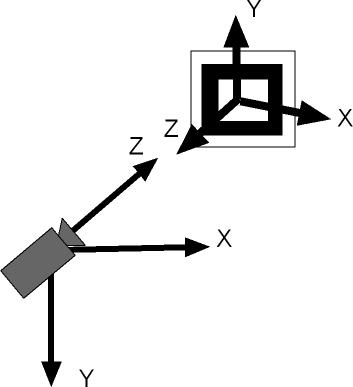
\includegraphics[width=0.6\columnwidth]{images/coordsys.jpg}
	\end{center}
	\caption{The \texttt{ARToolKit} coordinate systems for the camera and the identified pattern.}
	\label{fig:coordsys}
\end{figure}

To achieve the rotation of the camera, at the beginning of each frame the transformation matrix ($T$) is multiplied by the direction vector ($d$) and the up vector ($u$), generating the computed versions ($d'$ and $u'$, respectively).\footnote{The default values are used in the multiplication, otherwise the pattern would act like a steering wheel in a continuous camera movement. This would imply adding much complexity to the solution to  allow some control over the velocity, and would most probably bring back the difficulties found in the previous stage with the Euler angles.}. Any translation of $\Delta s$ space units to be performed since the computation of the last frame is applied to the position vector $p$ along the computed direction $d'$. This same vector $d'$ is then used to define the target position $t$ at a distance of $z$ space units from the camera. These computed values are the ones passed to the \texttt{lookAt} function. 

\begin{IEEEeqnarray}{rCl}
d' & = & T \times d 	\nonumber	\\
u' & = & T \times u 	\nonumber	\\
t  & = & p + d' * z	\nonumber	\\
p & = & p + d' * \Delta s 	\nonumber
\end{IEEEeqnarray}

The camera control is tested in a scene with various teapots in a cube shape around the origin of the world coordinate system. To draw the teapots, different shaders are used to change the colors. Each teapot receives a color related to its position in the cube:
\begin{enumerate}
\item{\textbf{Red} for the teapots in the faces intersected by the $x$ axis;}
\item{\textbf{Green} for those in the faces intersected by the $y$ axis;}
\item{\textbf{Blue} for the ones in the faces intersected by the $z$ axis.}
\end{enumerate}
The teapots in the edges receive the color from both faces they belong to, and the ones in the corners are drawn in white. All the shaders use Phong's algorithm lit from a point in space. The light and placement of the teapots help in recognizing the camera's movement, while the color system allows for some orientation while testing, so the viewer is able to distinguish the various possible movements.

\begin{figure}[!htp]
	\begin{center}
		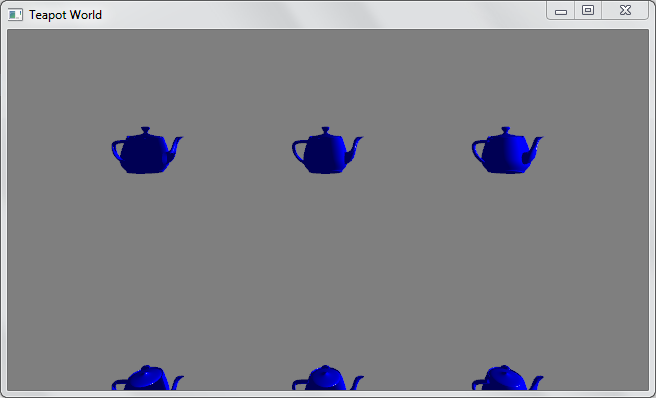
\includegraphics[width=\columnwidth]{images/screenshot/default.png}
		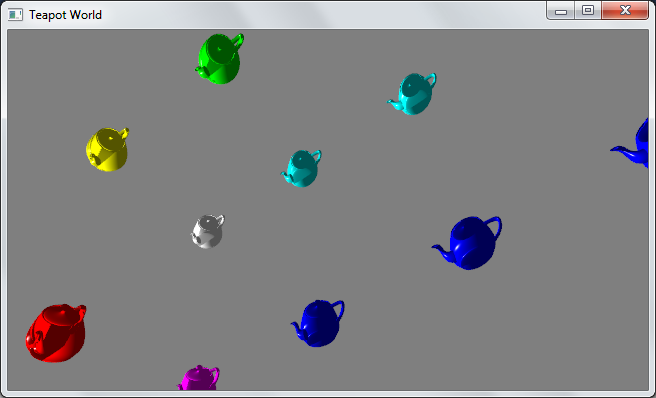
\includegraphics[width=\columnwidth]{images/screenshot/ftl.png}
	\end{center}
	\caption[Application screenshots]{Screenshots of the working application. On top, the default view (camera looking in the negative $z$ direction); below, the view with the pattern pointing to the frontal top left corner of the cube (negative $x$, positive $y$, negative $z$).}
	\label{fig:screenshots}
\end{figure}

\section{Conclusion}
This document presented the implementation of a 3-D world scene with a vision controlled perspective. The implemented system uses the \texttt{ARToolKit} library to recognize the pattern and applies its orientation to the virtual camera, successfully allowing the viewer to ``look around'' in the 3-D world.

Although not implemented in the current version, this system supports a navigation system which may or may not be independent of the pattern orientation. Using abstract vectors instead of only points, it becomes trivial to implement movement along the direction of the camera for example. Such features were not implemented only due to time constraints.

Before reaching the current stage, two distinct solutions were prepared to answer this stage of the Integrated Project, but each implemented a system different than the one intended. The reason for this to happen was the lack of a guiding example, or a text describing the assignment. Although the simplicity of the project allowed to keep correcting, the misinterpretations which arised from this resulted in a heavy time consumption preparing code and studying approaches which will be ignored in any evaluation process.

Any future work on this system will start by implementing the mentioned navigation system, as the only challenge is in deciding if and how the implemented vision system would interact with the navigation. The system can move in the direction the camera is looking, or both systems can be made completely apart allowing the viewer to change the camera's position while ``looking around''.

\end{document}
